\chapter{Evaluierung der Verwendbarkeit des Werkzeugs} % (fold)
\label{cha:eval_werkzeug}

Im ersten empirischen Teil der Evaluierung wurde die grundlegende Verständlichkeit und Verwendbarkeit des Werkzeug geprüft. Ziel war es hier, konzeptionelle und technische Eigenschaften bzw. Verhaltensweisen des Werkzeugs zu identifizieren, die den Modellierungsprozess behindern oder unterbrechen. Darunter fällt grundsätzlich jede Eigenschaft und jede Verhaltensweise, die die Benutzer zwingt, sich mit dem technischen System an sich zu beschäftigen und von der Erfüllung der eigentlichen Aufgabe ablenkt bzw. diese unterbricht.

Die Untersuchung wurde daneben auch genutzt, um explorativ die inhaltliche Verwendung des Systems zu untersuchen (d.h. wie es für seinen eigentlichen Verwendungszweck, die Modellierung, eingesetzt wurde) und Hypothesen abzuleiten, die in weiteren Schritten getestet werden konnten.

\section{Hypothesen} % (fold)
\label{sec:hypothesen}

In diesem Abschnitt werden die Hypothesen angeführt und begründet, die in diesem Teil der empirischen Untersuchung geprüft werden. Die hier angegebenen Hypothesen gehen auf die Eigenschaften des Werkzeugs in der Verwendung durch die Benutzer ein. Bei der Hypothesenbildung wird auf den Verwendungszweck des Werkzeugs, die Unterstützung der Bildung diagrammatischer Modelle, Rücksicht genommen -- die Modelle selbst sind jedoch nicht Gegenstand der Betrachtung, sondern werden erst im nächsten Kapitel behandelt. Nicht berücksichtigt wird außerdem die Verwendung zur Unterstützung von Articulation Work -- die Implikationen des Werkzeugs auf diese sind Gegenstand von Kapitel \ref{cha:eval_aw}.

\subsection{Konzeptionell begründete Hypothesen} % (fold)
\label{sub:konzeptionell_begründete_hypothesen}

Die folgenden Hypothesen wurden aus der Aufgabenstellung (siehe Kapitel \ref{cha:einführung}) sowie den Anforderungen an das Werkzeug (siehe Kapitel \ref{cha:anforderungen}) abgeleitet. Neben der Formulierung der Hypothese ist jeweils die Begründung aus der Konzeption des Werkzeugs angeführt.

Der grundlegende Anspruch des Werkzeugs ist es, explizite Articulation Work zu unterstützen. Wie in Teil \ref{prt:grundlagen} dieser Arbeit beschrieben, wird dies hier über die Externalisierung und Aushandlung von mentalen Modellen realisiert. Ein gängiges Mittel, um mentale Modelle zu repräsentieren, sind diagrammatische Modelle, worunter die Ergebnisse der vorgeschlagenen Methoden zur Externalisierung -- Concept Mapping und Strukturlegetechniken -- fallen. Das Werkzeug muss also die Repräsentation diagrammatischer Modelle unterstützen. 

\begin{hyp}
	\label{hyp:diagmodelle}
	Das Werkzeug ermöglicht die Repräsentation diagrammatische Modelle.
\end{hyp}

„Articulation Work“ ist immer in einen kooperativen Arbeitszusammenhang eingebettet. Die Kollaboration findet dabei nicht nur im produktiven Teil der Arbeit statt, sondern hat immer auch Auswirkungen auf die „Articulation Work“. Jede Unterstützung von „Articulation Work“ muss damit auch in kooperativen Szenarien einsetzbar sein. Dies gilt auch für das hier vorgestellte Werkzeug, das die kooperative Bearbeitung einer Aufgaben (hier: der Externalisierung und Abstimmung mentaler Modelle) ermöglichen muss. 

\begin{hyp}
	\label{hyp:kollaborativ}
	Das Werkzeug ermöglicht kooperatives Arbeiten an einer Aufgabe.
\end{hyp}

Die Aspekte von Arbeit, die im Rahmen von „Articulation Work“ abzustimmen sind, sind unterschiedlicher Natur. Naheliegend ist eine Abstimmung der Abläufe und Schnittstellen zwischen Personen, aber auch nicht-prozedurale Information wie das Verständnis der Struktur und Elemente eines Arbeitszusammenhangs kann Gegenstand von Articulation Work sein. Gleiches gilt für die im Rahmen der Articulation Work abzustimmenden mentalen Modelle -- diese bilden die Basis für Handlungsentscheidungen, umfassen aber im Allgemeinen (in Abgrenzung zu Schemata) nicht nur handlungsleitende Information sondern auch Kontextinformation, die die Bewertung der wahrgenommenen Situation ermöglicht. Demensprechend muss ein Werkzeug zu Unterstützung von expliziter Articulation Work und damit der Externalisierung von mentalen Modellen die Verwendung in unterschiedlichen Kontexten, d.h. für unterschiedliche zu externalisierenden Informationsstrukturen, die in mentalen Modellen abgebildet sind, ermöglichen.

\begin{hyp}
	\label{hyp:kontexte}
	Das Werkzeug ist gleichwertig für Modellierungsaufgaben in unterschiedlichen Kontexten einsetzbar.
\end{hyp}

Die ersten drei hier formulierten Hypothesen sind unmittelbar aus der globalen Zielsetzung abgeleitet und bilden die grundlegenden Anforderungen an das Werkzeug bei der Unterstützung von Articulation Work ab. Die nun folgenden Hypothesen sind konzeptionell nicht mehr direkt auf die globale Zielsetzung ausgerichtet sondern stellen auf Funktionalität des Werkzeugs ab, die den Modellbildungsprozess unterstützen soll. 

Die erste dieser Hypothesen bildet eine wesentliche Funktionalität des Werkzeugs, nämlich die Möglichkeit durch die Entstehungsgeschichte des erstellten Modells zu navigieren, ab. In der dieser Funktionalität zugrundeliegenden Literatur (\citep{Shipman00}, \citep{Klemmer02}) wird diese als wesentlich bezeichnet, wenn Externalisierungsprozesse unterbrochen werden, kollaborativ durchgeführt werden oder Dritten die Möglichkeit gegeben werden soll, die Entstehung des Modells nachzuvollziehen. Allen drei Aspekten liegt die Annahme zugrunde, dass in der Historie des Externalisierungsprozesses die dem Ergebnis zugrundeliegenden Ideen und Annahmen zu erkennen sind. Im Kontext dieser Arbeit bedeutet dies, dass aus der Nachverfolgung der Historie des externalisierten Modells die diesem zugrundeliegenden mentalen Modelle verständlich und nachvollziehbar werden. 

\begin{hyp}
	\label{hyp:historie}
	Die Reflexion des Modellierungsverlaufs ermöglicht das Verständnis der dem Modell zugrundeliegenden mentalen Modelle.
\end{hyp}

Auf Basis der Möglichkeit zur Navigation durch die Entstehungsgeschichte des Modells besteht auch die Möglichkeit, vergangene Modellzustände wiederherzustellen. Das Werkzeug unterstützt dabei die Benutzer durch die Ausgabe von schrittweisen Anweisungen, die den aktuellen Modellzustand in den wiederherzustellenden Zustand überführen. Allgemein bietet diese Funktionalität die Möglichkeit, erkannte Fehler im Modell zu korrigieren, ohne dabei bereits repräsentierte Information zu verlieren. Im kollaborativen Einsatz ermöglicht diese Funktionalität, alternative, individuelle Sichten auf den abzustimmenden Sachverhalt zu repräsentieren und dabei die Möglichkeit bieten, einen für alle Beteiligten akzeptablen Ausgangspunkt wiederherzustellen

\begin{hyp}
	\label{hyp:wiederherstellung}
	Die Möglichkeit der Wiederherstellung vergangener Modellzustände fördert die Bereitschaft alternative Repräsentationen auszuprobieren.
\end{hyp}

Die letzten beiden Hypothesen dieses Abschnitts sind ausschließlich auf die Verwendung des Werkzeugs an sich ausgerichtet und stehen nicht im Kontext von Articulation Work oder der Unterstützung der Externalisierung mentaler Modelle. Hypothese \ref{hyp:behinderung} steht für den in der Zielsetzung formulierten Anspruch, dass das Werkzeug in den Hintergrund treten muss und die Beschäftigung mit der eigentlichen Aufgabe nicht behindern darf. Dabei wird hier nicht auf den konkreten Anwendungsfall -- die Erstellung von Modellen -- eingegangen sondern lediglich die allgemeine Funktionsfähigkeit und Bedienbarkeit des Werkzeugs betrachtet. Ersteres ist Gegenstand der Evaluierung der erstellten Modelle, die in Kapitel \ref{cha:eval_modell} beschrieben werden.

\begin{hyp}
	\label{hyp:behinderung}
	Das Werkzeug behindert die Modellbildung nicht.
\end{hyp}

Hypothese \ref{hyp:gewöhnung} geht davon aus, dass bei wiederholten Verwendung des Werkzeugs Lern- und Gewöhnungseffekte auftreten, die die Verwendung erleichtern, beschleunigen und zu weniger Fehlbedienung führen. Dies ist ein Effekt, der bei jedem Werkzeug zu erwarten ist, dessen zugrundeliegenden Konzepte den Benutzern bewusst sind. Von dieser Voraussetzung kann durch die inhaltliche Einführung der Benutzer in die das Werkzeug prägenden und motivierenden Ideen ausgegangen werden. Damit wäre zu erwarten, dass das Werkzeug bei wiederholtem Einsatz in den späteren Anwendungen effizienter (im Sinne von schneller und Fehlbedienungen vermeidend) verwendet wird.

\begin{hyp}
	\label{hyp:gewöhnung}
	Wiederholte Verwendung des Werkzeugs führt zu schnellerer Modellbildung und weniger Fehlbedienungen.
\end{hyp}

% subsection konzeptionell_begründete_hypothesen (end)

\subsection{Explorativ gebildete Hypothesen} % (fold)
\label{sub:explorativ_gebildete_hypothesen}

Neben den aus der Aufgabenstellung abgeleiteten Hypothesen wurden einige Hypothesen auch während der Durchführung der einzelnen Evaluierungs-Blöcke gebildet. Diese Hypothesen sind spezifischer auf einzelne Aspekte des Werkzeugs abgestellt und decken beobachtete Auffälligkeiten und Missverständnisse in der Verwendung des Werkzeugs ab. 

Die erste in diesem Zusammenhang beobachtete Auffälligkeit betrifft die Herstellung von Verbindern zwischen einzelnen Modellelementen. Wie in Abschnitt \ref{sub:verbinden_von_modellelementen} beschrieben, existieren zwei Möglichkeiten, diese Funktion auszuführen. Einerseits können die beiden Modellelemente, die verbunden werden sollen, mit Markierungs-Tokens ausgewählt werden, worauf hin eine Verbindung hergestellt werden. Andererseits können Verbinder auch durch das Zusammenführen der zu verbindenden Blöcke (bis sich deren Breitseiten berühren) hergestellt werden. In der ersten Implementierung des Werkzeugs, die im Evaluierungs-Block 1 und im ersten Teil des zweiten Blocks verwendet wurde, war lediglich die erste Variante verfügbar. Die Möglichkeit zur Herstellung von Verbindern wurde in den in diesen Blöcken durchgeführten Anwendungen kaum eingesetzt. Dies führte einerseits zur Bildung der Hypothese \ref{hyp:keineverbinder} (siehe Abschnitt \ref{sub:m_explorativ_gebildete_hypothesen}), andererseits wurde bei ersten Auswertungen der Beobachtungen der im Verhältnis zum übrigen Modellierungs-Prozess hohe Zeit-Aufwand bei der Herstellung von Verbindern offensichtlich. Dieser Aufwand ist den Maßnahmen zur Stabilisierung der Erkennungsleistung des Werkzeugs geschuldet und kann mit den eingesetzten Interaktionsablauf nicht reduziert werden. Aufgrund einer Anregung eines Untersuchungsteilnehmers wurde deshalb die oben beschriebene zusätzliche Möglichkeit zur Herstellung von Verbindungen implementiert. Zu untersuchen ist nun, ob diese Maßnahme die Nutzung von Verbindern bei der Modellbildung tatsächlich erhöht.

\begin{hyp}
	\label{hyp:verbinder}
	Die Einführung der alternativen Möglichkeit zur Verbindungsherstellung erhöht die Nutzung von Verbindern bei der Modellerstellung.
\end{hyp}

Die zweite hier aufgestellte Hypothese betrifft eine Auffälligkeit bei der Verwendung des Löschtokens. Das Löschtoken wird verwendet, um das Werkzeug in einen Modus zu versetzen, in dem Verbinder gelöscht werden können. Schon die konzeptionelle Einordnung des Werkzeugs in Kapitel \ref{cha:konzeptionelle_evaluierung} zeigte Potential für Missverständnisse in der Verwendung dieses Tokens (siehe z.B. die Abschnitte \ref{sec:spezifikation_des_tac_schemas_nach_shaer_et_al_} und \ref{sec:einordnung_in_die_taxonomie_von_fishkin}). Zusammengefasst liegt die aus der Theorie ableitbare Problematik darin, dass durch die äußere Form des Tokens -- einem Radiergummi -- eine Metapher für dessen Verwendung („ausradieren“ von Elementen) suggeriert wird, die in dieser Form im Werkzeug nicht umgesetzt ist, da das Token lediglich als Schalter fungiert. Erste Beobachtungen deuteten darauf hin, dass die Verwendung des Löschtoken tatsächlich unverständlich oder missverständlich zu sein scheint. Die zugehörige Hypothese ist positiv formuliert, zu erwarten wäre demnach, dass sie verworfen werden muss.

\begin{hyp}
	\label{hyp:radierer}
	Das Löschtoken ermöglicht intuitives Löschen von Modellelementen.
\end{hyp}

% subsection explorativ_gebildete_hypothesen (end)
% section hypothesen (end)

\section{Untersuchungsdesign und Durchführung} % (fold)
\label{sec:untersuchungsdesign}

In diesem Abschnitt wird auf Basis der eben formulierten Hypothesen ein Untersuchungsdesign abgeleitet und die Durchführung der Untersuchung beschrieben. Im ersten Schritt werden die Hypothesen hinsichtlich der Möglichkeiten ihrer Beurteilung betrachtet und dabei die zu erhebenden Variablen identifiziert. Im nächsten Schritt folgt die Operationalisierung, in der die konkrete Messung bzw. Beurteilung der einzelnen Variablen festgelegt wird. Aus dieser Operationalisierung können die durchzuführenden Untersuchungen abgeleitet werden. An dieser Stelle erfolgt auch die Einordnung in die in Kapitel \ref{cha:eval_ueberblick} beschriebenen Evaluierungsblöcke. Im letzten Teil dieses Abschnitts wird die eigentliche Durchführung beschrieben, wobei im Speziellen auf deskriptive Parameter der Untersuchung eingegangen wird, die im Kontext der Werkzeugverwendung von Interesse sind, aber nicht oder nur als Teil der Berechnungsgrundlage in die Auswertung der Hypothesen eingehen.

\subsection{Operationalisierung} % (fold)
\label{sub:operationalisierung}

In diesem Abschnitt wird für jede Hypothese identifiziert, in welcher Form sie geprüft werden kann. Dies umfasst die Festlegung der Messpunkte sowie der jeweiligen Mess- und Auswertungsmethode (letzte bezugnehmend auf den in Abschnitt \ref{sec:eingesetzte_werkzeuge_und_verfahren} beschriebenen Verfahren). Zudem werden jene Evaluationsblöcke festgelegt, die für die jeweilige Untersuchung herangezogen wurden.

Für jede Hypothese wird also spezifiziert, anhand welcher Aspekte diese geprüft werden kann (= abhängige Variablen). Zudem wird festgelegt welche Ausgangssituation bei der Anwendung gewählt werden muss, um die Prüfung durchführen zu können (= unabhängige Variable) und welche Faktoren die Beurteilung ggf. ungewollt beeinflussen können (= Störvariablen).

\subsubsection{Repräsentation diagrammatischer Modelle} % (fold)
\label{ssub:repräsentation}

Gegenstand dieses Abschnitts ist die Prüfung der Hypothese \ref{hyp:diagmodelle}. Diese bezieht sich auf die Eignung des Werkzeugs für die Repräsentation diagrammatischer Modelle.

Voraussetzung für die Prüfung der Hypothese ist der Einsatz von Modellierungsaufgaben, die so formuliert sind, dass es grundsätzlich möglich ist, sie durch die Beschreibung in einem diagrammatischen Modell zu erfüllen. Keinen Einfluss auf die Untersuchung haben die eingesetzte Methodik sowie eventuell vorhandene Modellierungsvorkenntnisse, da die grundsätzlich Möglichkeit der Erstellung diagrammatischer Modelle unabhängig von der Art der Verwendung und von der Kompetenz der Benutzer ist. 

Geprüft wird die Hypothese hier an der \emph{Repräsentation}, die mit Hilfe des Werkzeugs erstellt wurde. Ein diagrammatisches Modell zeichnet nach \citep{Larkin87} aus, dass in ihm Konzepte und deren Zusammenhänge visuell-graphisch dargestellt werden können (in Abgrenzung zu textuellen Beschreibungen). Zur Bewertung der Hypothese werden deshalb die erstellten Repräsentationen herangezogen und überprüft, ob sie den Anforderungen an ein diagrammatisches Modell -- das Vorhandensein von Konzepten und Beziehungen zwischen diesen -- erfüllen.

% subsubsection repräsentation (end)

\subsubsection{Kooperatives Arbeiten} % (fold)
\label{ssub:kollaboratives_arbeiten}

Gegenstand dieses Abschnitts ist die Prüfung der Hypothese \ref{hyp:kollaborativ}. Dabei wird überprüft, ob das Werkzeug kooperatives Arbeiten an einer Modellierungsaufgabe erlaubt.

Dazu muss eine Modellierungsaufgabe gewählt werden, die kollaboratives Arbeiten sinnvoll ermöglicht. Etwaige Modellierungsvorkenntnisse haben keinen Einfluss auf die Beurteilung der hier betrachteten Hypothese.

Zur Beurteilung eignen sich in diesem Fall die \emph{Zeitverteilung der Beteiligung} der einzelnen Benutzer am Modellierungsvorgang, das \emph{Verhalten der Benutzer bei simultaner Manipulation} eines Modells auf der Modellierungsoberfläche sowie der \emph{subjektive Eindruck der Benutzer} über deren Kooperation untereinander. Der erstgenannte Aspekt kann quantitativ gemessen werden, wobei eine tendenziell zeitlich gleichverteilte Einbindung der Beteiligten in die Modellbildung für die Annahme der Hypothese spricht. Zusätzlich kann mittels dem dritten und vierten Aspekt qualitativ beurteilt werden, ob und wie eine kooperative Manipulation des Modells durch mehrere Benutzer gleichzeitig möglich ist.

% subsubsection kollaboratives_arbeiten (end)

\subsubsection{Einsetzbarkeit in unterschiedlichen Kontexten} % (fold)
\label{ssub:einsetzbarkeit_in_unterschiedlichen_kontexten}

Gegenstand dieses Abschnitts ist die Operationalisierung der Hypothese \ref{hyp:kontexte}. Diese Hypothese zielt dabei auf die Eignung des Werkzeugs zur Modellbildung in unterschiedlichen Kontexten, d.h. für unterschiedliche Modellierungsaufgaben. 

Die \textbf{unabhängigen Variablen} sind dabei wiederum das \emph{Werkzeug} und die \emph{Methodik}, die wie konzipiert eingesetzt werden, sowie die \emph{Modellierungsaufgabe}, als jene Variable, die im Zuge der Untersuchung variiert wird. Etwaige \emph{Modellierungsvorkenntnisse} können insofern als \textbf{Störvariable} wirken, als das sie die Wahrnehmung der Eignung des Werkzeugs für eine bestimmte Aufgabe positiv oder negativ beeinflussen.

\textbf{Abhängige Variablen} sind in diesem Fall die \emph{Wahrnehmung der Eignung} durch die Benutzer, die qualitativ beurteilt wird, und die \emph{Korrelation der Größe der erstellten Modelle mit der benötigten Modellierungsdauer}. Korrelliert die Modellgröße positiv mit der Modellierungsdauer, so ist der Zeitanteil, der zu Beschäftigung mit dem Werkzeug selbst (und nicht mit der Modellierungsaufgabe) tendenziell stabil. Daraus kann abgeleitet werden, dass das Werkzeug die verglichenen Modellierungsaufgaben gleich gut (oder schlecht) unterstützt.

% subsubsection einsetzbarkeit_in_unterschiedlichen_kontexten (end)

\subsubsection{Reflexion des Modellierungsverlaufs} % (fold)
\label{ssub:reflexion_des_modellierungsverlaufs}

Gegenstand dieses Abschnitts ist die Operationalisierung der Hypothese \ref{hyp:historie}. Dabei wird überprüft, ob die Möglichkeit zur Reflexion des Modellierungsverlaufs das Verständnis der zugrundeliegenen mentalen Modelle ermöglicht bzw. verbessert.

Sowohl \emph{Werkzeug} und \emph{Methodik} sind als \textbf{unabhängige Variablen} zu identifizieren. Die Modellierungsaufgabe und Modellierungsvorkenntnisse haben keine Auswirkung auf die Untersuchung.

Als \textbf{abhängige Variable} kann hier der \emph{wahrgenommene Erfolg bei der Vermittlung eines mentalen Modells} herangezogen werden. Zur Beurteilung desselben wird eine Modellierungssituation geschaffen, in der eine Person für sich individuell das Werkzeug zur Externalisierung eines mentalen Modells benutzt. In einem zweiten Schritt wird eine zweite, zuvor nicht beteiligte Person aufgefordert, den Inhalt der auf der Modellierungsoberfläche vorhandenen Repräsentation zu interpretieren, wobei der Modellierungsverlauf herangezogen werden darf, eine Interaktion mit dem ursprünglichen Modellierer jedoch nicht gestattet ist. Im dritten Schritt beurteilt der ursprüngliche Modellierer die Adäquatheit der Interpretation und trifft so eine Aussage über den Erfolg des Transfers des mentalen Modells. In Kombination mit der Information über Art und Ausmaß der Benutzung der Möglichkeit zum Zugriff auf den Modellierungsverlaufs lässt sich eine qualitative Aussage über die Effekte dieser Funktionalität treffen.    

% subsubsection reflexion_des_modellierungsverlaufs (end)

\subsubsection{Wiederherstellung vergangener Modellzustände} % (fold)
\label{ssub:wiederherstellung_vergangener_modellzustände}

Gegenstand dieses Abschnitts ist die Operationalisierung der Hypothese \ref{hyp:wiederherstellung}. Gegenstand der Überprüfung ist die Verwendung der Wiederherstellungsfunktionalität zum Zwecke der versuchsweisen Veränderung des Modells.

Als \textbf{unabhängige Variablen} wirken hier wie zuvor \emph{Werkzeug} und \emph{Methodik}, die \emph{Modellierungsaufgabe} hat insofern Auswirkungen, als dass sie so gestaltet sein muss, dass sinnvoll unterschiedliche Repräsentationen gebildet werden können. Modellierungsvorkenntnisse haben keine Auswirkungen auf diese Untersuchung.

Die \textbf{abhängige Variable}, die zur Beurteilung dieser Hypothese herangezogen wird, ist die \emph{Anzahl der Verwendungen der Wiederherstellungsfunktionalität zur Korrektur inhaltliche verworfener Repräsentationen}. Höhere Werte deuten hier auf eine Annahme der Hypothese hin. Zusätzlich können qualitative Aussagen zur Nutzung dieser Funktionalität und deren \emph{wahrgenommenen Nutzen} zur Beurteilung verwendet werden. 

% subsubsection wiederherstellung_vergangener_modellzustände (end)

\subsubsection{Nicht-Behinderung} % (fold)
\label{ssub:nicht_behinderung}

Gegenstand dieses Abschnitts ist die Operationalisierung der Hypothese \ref{hyp:behinderung}. Dabei wird überprüft, ob bei der Verwendung des Werkzeugs dieses in den Aufmerksamkeitsfokus der Benutzer tritt oder sich diese auf die eigentliche Modellierungsaufgabe konzentrieren können. 

\textbf{Unabhängige Variablen} sind in diesem Fall das \emph{Werkzeug} und die angewandte \emph{Modellierungsmethode}. Die Modellierungsaufgabe hat keinen Einfluss auf die Überprüfung dieser Hypothese, lediglich etwaig vorhandene \emph{Modellierungsvorkenntnisse} können als \textbf{Störvariable} wirken, da sie Einfluss auf die erwartete Funktionalität des Werkzeugs haben kann.

Zur Beurteilung, ob bzw. inwieweit das Werkzeug die Modellbildung behindert, werden qualitative beurteilbare \textbf{abhängige Variablen} herangezogen.  Die Anzahl von \emph{Fehlfunktionen des Werkzeugs} bzw. das \emph{Auftreten von Systemabstürzen} als Indikator für eine behindernde Wirkung des Werkzeugs herangezogen werden. Das Auftreten von Missverständnissen und daraus resultierende Fehlbedienungen können ebenfalls eine Behinderung des Modellierungsvorgangs interpretiert werden. Zudem wird das artikulierte Empfinden der Benutzer als Maß für die wahrgenommene Behinderung durch das Werkzeug herangezogen. Der Einfluss von Modellierungsvorkenntnissen kann in diesem Fall nicht mit rechnerischen Maßnahmen kompensiert werden. Etwaige Vorkenntnisse werden dementsprechend bei der Auswertung angeführt und müssen bei der Diskussion der Hypothese berücksichtigt werden.

% subsubsection nicht_behinderung (end)

\subsubsection{Gewöhnung an das Werkzeug} % (fold)
\label{ssub:gewöhnung_an_das_werkzeug}

Gegenstand dieses Abschnitts ist die Operationalisierung der Hypothese \ref{hyp:gewöhnung}. Dabei wird überprüft, ob wiederholte Benutzung des Werkzeugs Auswirkung auf die Qualität der Interaktion hat. Eine Erhöhung der Qualität äußert sich in schnellerer Modellbindung und weniger Fehlbedienung.

\textbf{Unabhängige Variablen} sind in diesem Fall \emph{die Verwendung des Modellierungswerkzeugs} und die angewandte \emph{Methodik}. \textbf{Störvariablen}, die unerwünschten Einfluss auf die Messung haben, sind potentiell die \emph{Modellierungsaufgabe} (die Einfluss auf die Dauer der Anwendung hat und außerdem die Verwendung unterschiedlicher Funktionalität bedingen kann) und eine etwaige \emph{veränderte Funktionalität des Werkzeugs} zwischen den verglichenen Evaluierungsblöcken (die die Interaktion einerseits erleichtern kann, andererseits aber auch zu Fehlbedienung aufgrund von unbekannten Interaktionsmustern führen kann). 

Die \textbf{abhängigen Variablen} zur Beurteilung der Qualität der Interaktion sind einerseits die \emph{Anzahl der Fehlbedienungen} des Werkzeugs pro Zeiteinheit und andererseits die \emph{Arbeitsdauer am Werkzeug}\footnote{Die Arbeitsdauer am Werkzeug ist im Gegensatz zur gesamten Modellierungsdauer um jenen Zeitanteil reduziert, in dem die Teilnehmer interagieren, ohne am Werkzeug zu arbeiten.} in Abhängigkeit der Modellgröße. Die Normierung der abhängigen Variablen ist notwendig, um vergleichbare Werte für unterschiedliche Werkzeug-Anwendungen zu erhalten. Sinken beide Werte zwischen zwei Evaluierungsblöcken, die auf der gleichen Stichprobe aufbauen, signifikant, so kann die Hypothese angenommen werden. Um den Einfluss der Störvariablen zu reduzieren, ist es sinnvoll, in beiden Blöcken eine identische Modellierungsaufgabe zu stellen und die Funktionalität des Werkzeugs nicht zu verändern. Identische Modellierungsaufgaben können durch die wiederholte inhaltliche Beschäftigung mit der Aufgabe zu schnellerer Arbeit bzw. zu kompakteren Modellen führen. Diesem weiteren Störfaktor kann durch die Berücksichtigung der reinen Arbeitszeit am Werkzeug sowie der Normierung derselben in Abhängigkeit der Modellgröße entgegengewirkt werden.

% subsubsection gewöhnung_an_das_werkzeug (end)

\subsubsection{Herstellung von Verbindern} % (fold)
\label{ssub:herstellung_von_verbindern}

Gegenstand dieses Abschnitts ist die Operationalisierung der Hypothese \ref{hyp:verbinder}. Mit Hilfe dieser Hyothese soll überprüft werden, ob die Einführung der alternativen Möglichkeit zur Herstellung von Verbindern deren Verwendung signifikant gesteigert hat.

Die für diese Hypothese relevanten \textbf{unabhängigen Variable} ist die \emph{Verwendung des Werkzeugs}. \textbf{Störvariablen} sind die \emph{Modellierungsaufgabe} (da sie die Anzahl der benötigten Verbinder beeinflussen kann), die \emph{Methodik} (da sie die Verwendung von Verbindern im Allgemeinen bedingen oder vermeiden kann) und \emph{eventuell vorhandene Modellierungsvorkenntnisse} (da diese Einfluss auf die Struktur des Modells haben können). Um den Einfluss deer Störvariablen zu reduzieren, wird die Messung zwischen zwei Evaluierungsblöcken vorgenommen, in denen die gleiche Stichprobe mit der gleichen Aufgabenstellung das Werkzeug mit der gleichen Methodik anwandte. Lediglich die Funktionalität des Werkzeugs wurde zwischen den beiden Anwendungen um den alternativen Weg zur Herstellung von Verbindern erweitert.  

Als \textbf{abhängige Variable} ist zur Beurteilung des Ausmaßes der Verwendung von Verbindern in diesem Fall die \emph{Connectedness} des Modells verwendbar. Die Connectedness ist das Verhältnis zwischen der Anzahl der im Modell verwendeten Verbinder und der Anzahl der verwendeten Knoten (Modellierungselemente). Hier ist zu prüfen, ob die Connectedness in jenem Evaluierungs-Block, in dem der alternative Weg zur Herstellung von Verbindungen verfügbar war, signifikant höher ist als in jenem Block, in dem sie nicht verfügbar war.

% subsubsection herstellung_von_verbindern (end)

\subsubsection{Löschtoken} % (fold)
\label{ssub:löschtoken}

Gegenstand dieses Abschnitts ist die Operationalisierung der Hypothese \ref{hyp:radierer}. Dabei wird überprüft, ob das Löschtoken intuitiv korrekt verwendet wird oder ob es zu Fehlinterpretationen kommt.

Die Verwendbarkeit des Löschtokens ist unabhängig von der Modellierungsaufgabe, der angewandten Methodik und auch von eventuell vorhandenen Modellierungsvorkenntnissen. Die einzig relevante \textbf{unabhängige Variable} ist die \emph{Verwendung des Werkzeugs} selbst. 

Zur Beurteilung der intuitiven Verwendbarkeit werden quantitative und qualitative Merkmale der Werkzeugverwendung herangezogen. Eine quantitativ beurteilbare \textbf{abhängige Variable} ist der Anteil der Fehlbedienungen des Löschtokens in Bezug auf alle Anwendungen des Werkzeugs, in denen es grundsätzlich verwendet wurde. Qualitativ wird die Art des Missverständnisses, das zu den jeweiligen Fehlbedienungen führt, beurteilt.

Zur Messung der quantitativen Variablen wird für jede Anwendung die Anzahl der Fehlbedienungen erhoben, die durch das Löschtoken verursacht wurden. Dieser Wert wird in Bezug zur Gesamtanzahl der Fehlbedienungen gesetzt, so dass der Anteil der durch das Löschtoken verursachten Fehlbedienungen berechnet werden kann. Bei "gleich guter" intuitiver Bedienbarkeit aller Werkzeuge wäre eine Gleichverteilung der Fehler zu erwarten. Ist der Anteil der durch das Löschtoken verursachten Fehlbedienungen höher als der Anteil, der bei Gleichverteilung zu erwarten wäre, so deutet dies auf eine Ablehnung der Hypothese hin.

Qualitativ werden Modellierungssituationen betrachtet, in denen das Löschtoken zum Einsatz kommt. Auf Basis von Transkripten der Interaktion zwischen den Benutzern und dem Werkzeug, bei denen es zu Fehlbedierungen kam, werden die aufgetretenen Missverständnisse explizit identifziert.

% subsubsection löschtoken (end)

% subsection operationalisierung (end)

\subsection{Datenbasis} % (fold)
\label{sub:datenbasis}

Als Grundlage der Überprüfung der Hypothesen werden hier die Evaluierungs-Blöcke 1 bis 5 verwendet. Dabei wurden für die quantitativ zu prüfenden Variablen die Blöcke 2 und 3 herangezogen. In die qualitative Auswertung der Ergebnisse wurden hingegen alle Blöcke (1-5) mit einbezogen.

% subsection datenbasis (end)

\subsection{Durchführung} % (fold)
\label{sub:durchführung}

In diesem Abschnitt werden die für diesen Evaluierungs-Teil relevanten deskriptiven Parameter der berücksichtigten Anwendungs-Blöcke angeführt.

\subsubsection{Stichprobe} % (fold)

\begin{tabular}{| p{2cm} || p{2,5cm} | p{2,5cm} | p{2,5cm} || p{2cm} |}
  \hline
   & Aushandlung (1. Durchgang) & Aushandlung (2. Durchgang) & Concept Mapping & Gesamt \\ \hline
   $n_{Anwendungen}$ & 9 & 9 & 17 & 35 \\ 
   $n_{Teilnehmer}$ & 19 & 18 & 47 & 84 \\ \hline
\end{tabular} 

\subsubsection{Dauer der Werkzeugverwendung} % (fold)

Die Dauer der Werkzeug-Verwendung wurde den Blöcken 2 („Aushandlung“) und 3 („Concept Mapping“) erhoben. Die Bearbeitungszeit ist wie folgt verteilt (siehe auch Abbildung \ref{fig:img_Evaluierung_usageTimeOverview}\footnote{In allen Boxplots gilt folgende Notation: 
\begin{itemize}
	\item breite horizontale Linie: Bereich zwischen 25\%- und 75\%-Quantil
	\item breite vertikale Linie: Median
	\item linke schmale Linie: Bereich zwischen 2,5\%- und 25\%-Quantil
	\item rechte schmale Linie: Bereich zwischen 75\%- und 97,5\%-Quantil
	\item Kreuze: Ausreißer (außerhalb 2,5\%- und 97,5\%-Quantil)
\end{itemize}
}):

\begin{tabular}{| p{1cm} || p{3cm} | p{3cm} | p{3cm} |}
  \hline
   & Aushandlung (1. Durchgang) & Aushandlung (2. Durchgang) & Concept Mapping \\ \hline
   $t_{min}$ & 11m 54s & 2m 5s & 14m 1s \\ 
   $\overline{t}$ & 20m 53s & 9m 49s & 32m 32s \\ 
   $s(t)$ & 4m 18s & 5m 20s & 10m 7s \\
   $t_{max}$ & 27m 30s & 19m 29s & 45m 0s \\ \hline
\end{tabular} 

\begin{figure}[htbp]
	\centering
		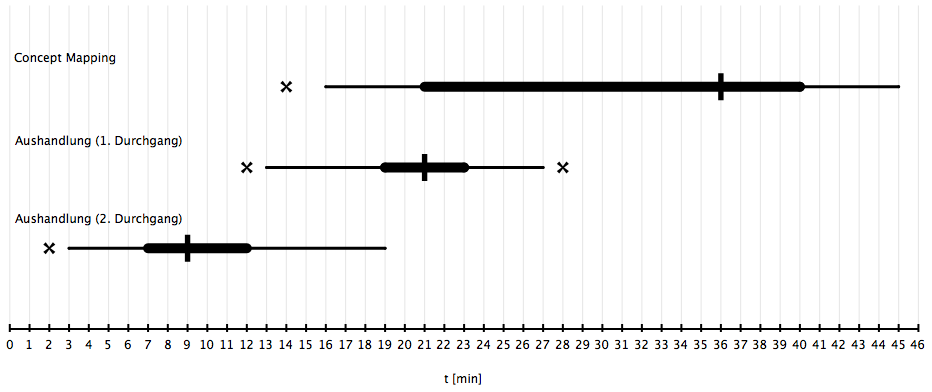
\includegraphics[width=15cm]{img/Evaluierung/usageTimeOverview.png}
	\caption{Dauer der Werkzeugverwendung -- Überblick}
	\label{fig:img_Evaluierung_usageTimeOverview}
\end{figure}

Die erhobene Dauer der Werkzeug-Verwendung teilt sich ein einen Anteil, an dem tatsächlich mit dem Werkzeug interagiert wird und einen Anteil, der anderen Tätigkeiten (wie inhaltlicher Diskussion, Bedeutungsaushandlung, \ldots) gewidmet ist. Diese beiden Anteile sind in den einzelnen Blöcken wie folgt verteilt (siehe auch die Abbildungen \ref{fig:img_Evaluierung_usageTimeConceptMapping} und \ref{fig:img_Evaluierung_usageTimeNegotiation}):

\begin{figure}[htbp]
	\centering
		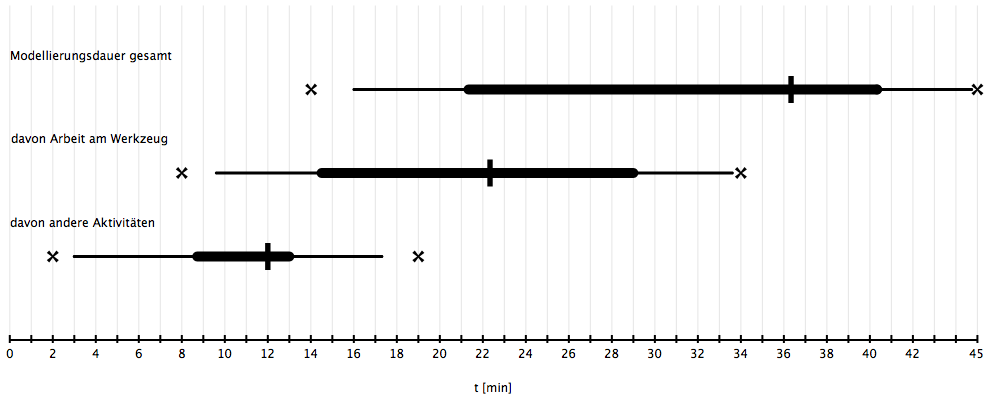
\includegraphics[width=15cm]{img/Evaluierung/usageTimeConceptMapping.png}
	\caption{Dauer der Werkzeugverwendung -- Concept Mapping}
	\label{fig:img_Evaluierung_usageTimeConceptMapping}
\end{figure}

\begin{figure}[htbp]
	\centering
		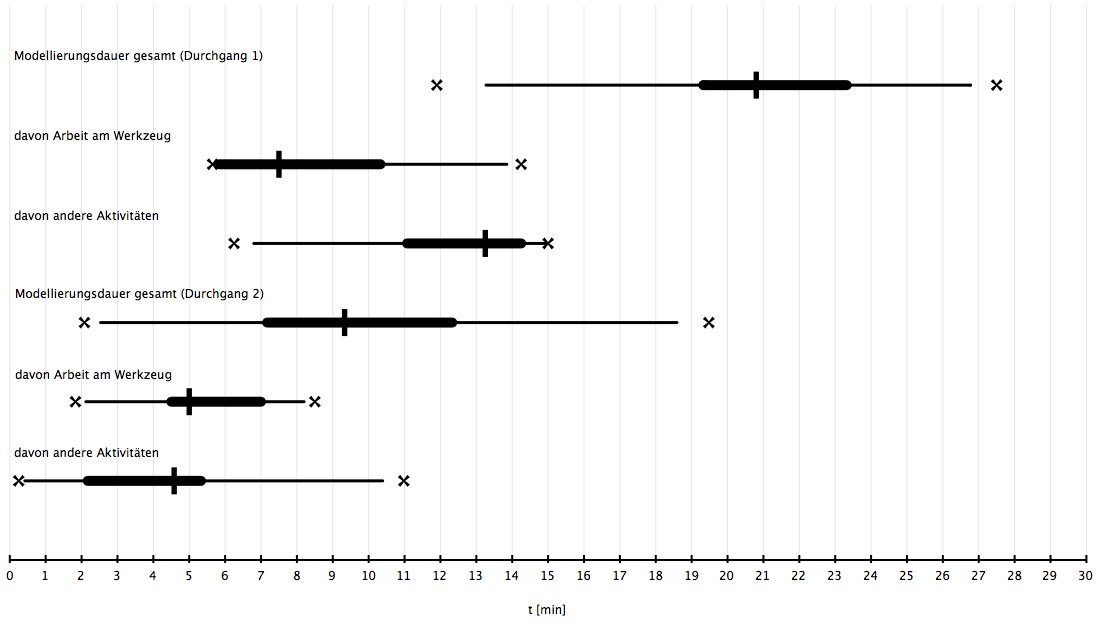
\includegraphics[width=15cm]{img/Evaluierung/usageTimeNegotiation.png}
	\caption{Dauer der Werkzeugverwendung -- Aushandlung}
	\label{fig:img_Evaluierung_usageTimeNegotiation}
\end{figure}

% subsection durchführung (end)
% section untersuchungsdesign (end)

\section{Ergebnisse} % (fold)
\label{sec:ergebnisse}

\subsection{Repräsentation diagrammatischer Modelle} % (fold)
\label{sub:repräsentation_diagrammatischer_modelle}

Gegenstand der hier beschriebenen Untersuchung Hypothese \ref{hyp:diagmodelle} („Das Werkzeug ermöglicht die Repräsentation diagrammatische Modelle.“). Als Grundlage dieser Untersuchung dienen die Ergebnisse aller Evaluierungsblöcke, da die Aufgaben in allen Fällen auf die Erstellung einer Repräsention in Form eines diagrammatischen Modells gefordert war.

Ausgewertet wird hier, ob die Ergebnisse der Modellierung jeweils als diagrammatisches Modell zu klassifizieren sind. Ein diagrammatisches Modell zeichnet nach \citep{Larkin87} aus, dass in ihm Konzepte und deren Zusammenhänge visuell-graphisch dargestellt werden. Eine Darstellung von Beziehungen kann durch die explizite Darstellung von Verbindungen zwischen Konzepten oder durch andere graphische Mittel wie Gruppierung von Konzepten in räumlicher Nähe erfolgen. Um eine eindeutige Auswertbarkeit gewährleisten zu können, wird hier auf die explizite Darstellung von Verbindungen eingeschränkt. 

\subsubsection{Auswertung} % (fold)

In allen vorliegenden Modellen wurden Konzepte als Grundelemente des diagrammatischen Modells verwendet. Das Kriterium zur Klassifizierung als diagrammatisches Modell ist im Folgenden also das Vorhandensein von Verbindungen.

\begin{tabular}{| p{3cm} || p{3cm} | p{3cm} |}
  \hline
   Block & Modelle gesamt & Modelle mit Verbindern \\ \hline
   1 & 9 & 0 \\ 
   2 & 17 & 9 \\ 
   3 & 18 & 17 \\ 
   4 & 9 & 9 \\ 
   5 & 11 & 11 \\ \hline
   Gesamt & 64 & 46 \\ \hline
\end{tabular}

Insgesamt sind in 64 Modellen, die als Ergebnis vorliegen 46 Modelle zu identifizieren, in denen explizit Verbindungen zur Darstellung von Beziehungen zwischen Konzepten verwendet werden ($71,9\%$). Eine implizite Darstellung von Beziehungen ist jedoch in allen vorliegenden Modellen zu erkennen. Nicht explizit durch Verbindungen abgebildete Beziehungen werden in allen Fällen durch die räumliche Konfiguration der Konzepte zueinander dargestellt.

\subsubsection{Diskussion} % (fold)

Legt man das Kriterium des Vorhandenseins von Verbindungen zwischen Konzepten an, so sind $71,9\%$ der betrachteten Modelle als diagrammatische Modelle zu klassifizieren. Dies erscheint vordergründig eine geringe Zahl zu sein, die gegen die allgemeine Gültigkeit der Hypothese sprechen würde. Allerdings sind in allen Modelle implizite Verbindungen zwischen Konzepten eindeutig zu identifizieren. Außerdem ist zu erkennen, dass der Anteil an diagramatischen Modellen über die Evaluierungsblöcke (und damit die Weiterentwicklung des Werkzeugs über die Zeit) hinweg stetig ansteigt, bis er in den letzten beiden Blöcken jeweils $100\%$ erreicht. Dies ist durch technische Fehlfunktionen zu erklären, die es in ersten Evaluierungsblöcken schwer bzw. teilweise unmöglich machten, explizite Verbindungen intentional zu erstellen. Unter Anbetracht dieser Erkenntnisse erscheint die Annahme der Hypothese \ref{hyp:diagmodelle} als gerechtfertigt.

Die Abbildung von Verbindungen durch räumliche Konfiguration ist Gegenstand der Prüfung von Hypothese \ref{hyp:keineverbinder} in Kapitel \ref{cha:eval_modell} und wird dort einer näheren Betrachtung unterzogen.

\subsubsection{Ergebnis} % (fold)

\textbf{Hypothese \ref{hyp:diagmodelle} kann in der Untersuchung angenommen werden.} Die Abbildung von Konzepten und Beziehungen zwischen diesen wurde in allen vorliegenden Modellen erfolgreich umgesetzt, wenngleich die Modellierung von expliziten Verbindungen in den ersten beiden Modellierungsblöcken aufgrund von technischen Unzulänglichkeiten nicht durchgeführt wurde.

% subsection repräsentation_diagrammatischer_modelle (end)

\subsection{Kollaboratives Arbeiten} % (fold)
\label{sub:kollaboratives_arbeiten}

Gegenstand der hier beschriebenen Untersuchung ist Hypothese \ref{hyp:kollaborativ} („Das Werkzeug ermöglicht kooperatives Arbeiten an einer Aufgabe.“). Zur Untersuchung der quantitativ beurteilbaren Aspekte wurden die Werkzeuganwendungen aus den Evaluierungsblöcken 2 ($n=9$) und 3 ($n=17$) herangezogen, wobei in Block 2 in Gruppen zu zwei Personen modelliert wurde (in einem Fall drei Personen), in Block 3 in Gruppen zu drei Personen (in drei Fällen nur zwei Personen). Zusätzlich wurden zur qualitative Beurteilung Daten aus Block 4 verwendet.

In Modellierungsblock 4 wurde hinsichtlich der subjektiven Wahrnehmung der Kooperation eine Befragung der Teilnehmer mittels eines Fragebogens durchgeführt (diese umfasste auch weitere Aspekte, die in späteren Abschnitten besprochen werden). Die Fragestellungen zur Kooperation wurde in 4 geschlossenen Items codiert, die auf einer 7-teiligen Likert-Skala zu beantworten waren. Zusätzlich wurden offene Fragen hinsichtlich der Nützlichkeit der Werkzeugs eingesetzt, die an dieser Stelle ebenfalls hinsichtlich Aussagen zur Kooperation zwischen den Teilnehmern ausgewertet werden.

\subsubsection{Auswertung} % (fold)

Grundlage des ersten Teils der Auswertung ist die Verteilung der Modellierungsdauer zwischen den Teilnehmern. Um die unterschiedliche Gesamt-Modellierungsdauer in den einzelnen Anwendungen zu kompensieren, wurden die Berechnungen auf Basis der prozentuellen Zeitanteile der einzelnen Teilnehmer durchgeführt. Die einzelnen Datensätze wurden so sortiert, dass die anteilsmäßige Modellierungsdauer von Teilnehmer A bis Teilnehmer C (bzw. B) abnimmt. In den einzelnen Evaluierungsblöcken ergeben sich die in Abbildung \ref{fig:img_Evaluierung_timeDist} dargestellten Verteilungen.

\begin{figure}[htbp]
	\centering
		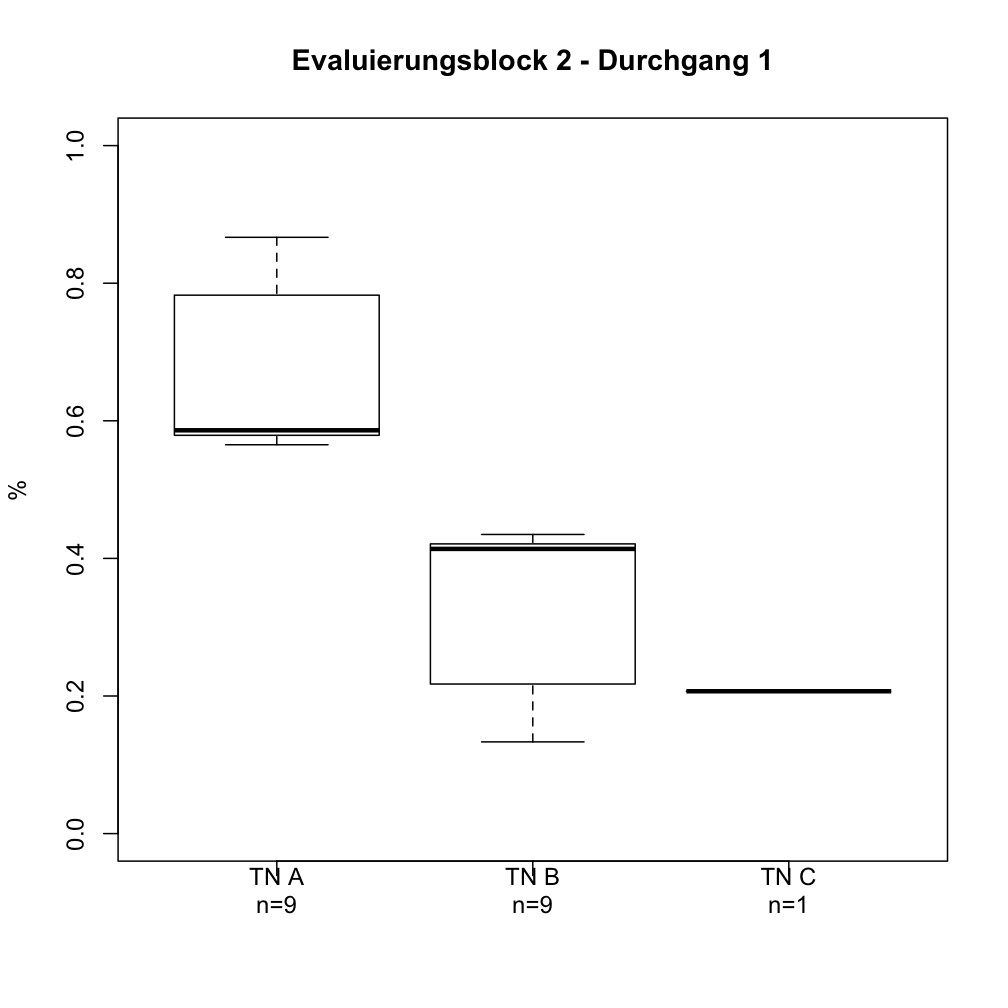
\includegraphics[height=2.5in]{img/Evaluierung/timeDistSE1.png}
		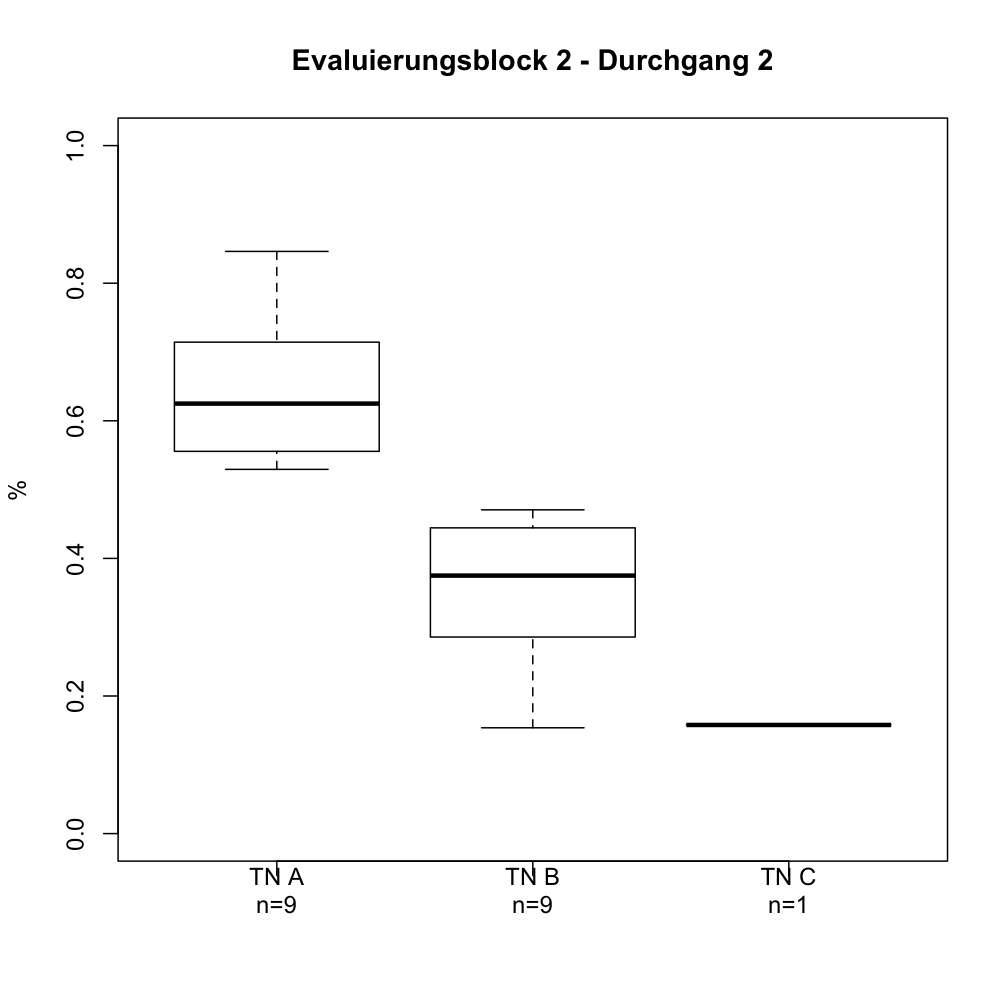
\includegraphics[height=2.5in]{img/Evaluierung/timeDistSE2.png}
		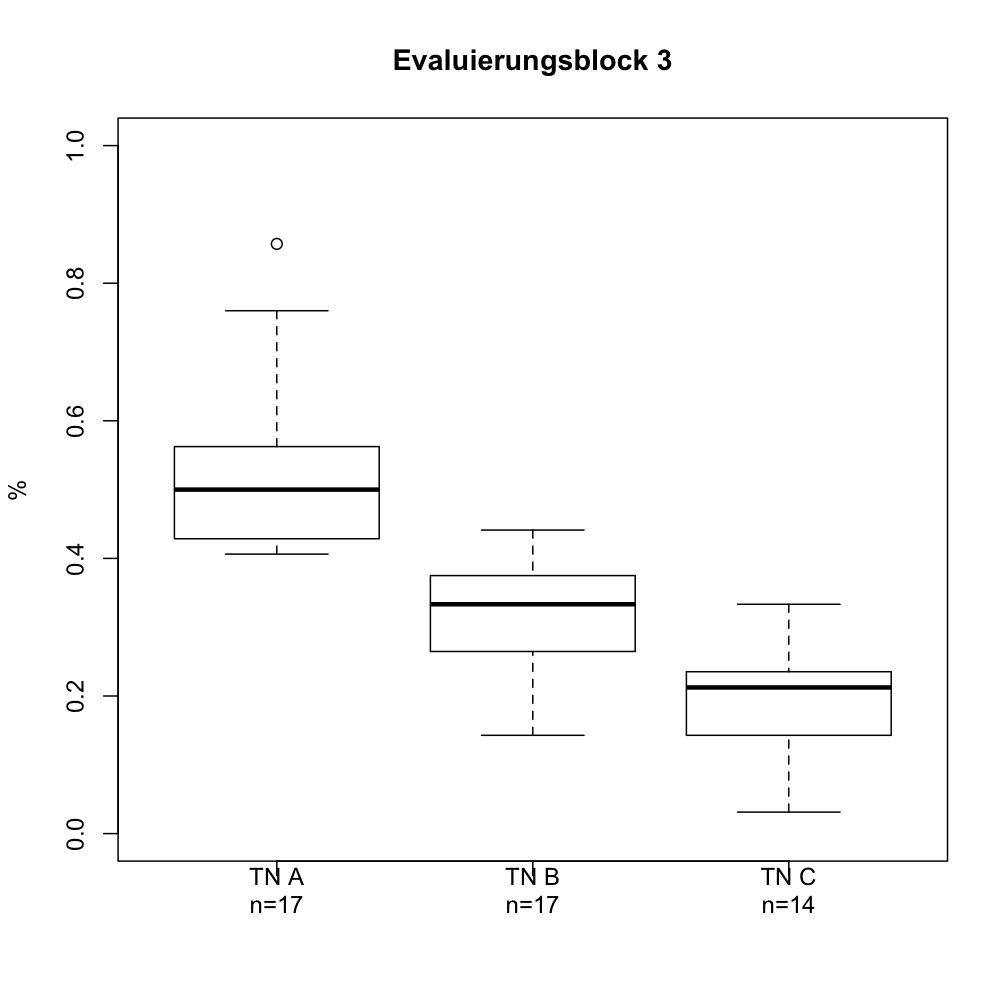
\includegraphics[height=2.5in]{img/Evaluierung/timeDistUE.png}
	\caption{Zeitverteilung zwischen den Teilnehmern}
	\label{fig:img_Evaluierung_timeDist}
\end{figure}

Zu prüfen ist hier, ob die Zeit-Anteile der einzelnen Teilnehmer signifikant unterschiedlich sind. Dazu wird für jeden Block die Signifikanz zwischen den Verteilung der einzelnen Teilnehmerklassen berechnet (eine Teilnehmerklasse setzt sich aus all jenen Teilnehmern zusammen, die am längsten, am zweitlängsten bzw. am drittlängsten aktiv waren).  Aufgrund der geringen Stichprobengröße kommt zur Prüfung der Signifikanz der t-Test nicht in Frage, es wird der \emph{Wilcoxon-Test} herangezogen. Der t-Test setzt außerdem Normalverteilung der Prüfgrößen voraus, was zumindest bei einer der Verteilungen nicht der Fall ist (Sharpiro-Wilk-Test für $conn_{B22}$: $p=6.29e^{-5}$, damit ist von Nicht-Normalverteilung auszugehen).

Im zweiten Teil der Auswertung wurde in einem Fragebogen in 4 Items aggregiert die Frage nach kooperativen Aspekten bei der Modellbildung gestellt. Diese wurden im Schnitt als sehr hoch oder hoch beurteilt ($M = 1.79$, $SD = 0.56$, $t4(13) = -14.28$, $p<.001$). Dieses Ergebnis steht in Übereinstimmung mit den qualitativen Aussagen der Benutzer, von denen 10 explizit auf die kooperationsfördende Wirkung des Werkzeugs hinwiesen. Auch in Auswertungen der  Videoaufnahmen der betreffenden Modellierungsdurchgänge ist zu erkennen, dass zwischen $40$ und $70\%$ der gesamten Modellierungsdauer der Interaktion zwischen den Teilnehmern zuzurechnen ist.

\subsubsection{Diskussion} % (fold)

\subsubsection{Ergebnis} % (fold)

% subsection kollaboratives_arbeiten (end)

\subsection{Herstellung von Verbindern} % (fold)
\label{sub:herstellung_von_verbindern}

Gegenstand der hier beschriebenen Untersuchung ist Hypothese \ref{hyp:verbinder} („Die Einführung der alternativen Möglichkeit zur Verbindungsherstellung erhöht die Nutzung von Verbindern bei der Modellerstellung.“). Zur Untersuchung herangezogen wurden die Werkzeuganwendungen aus Evaluierungsblock 2 ($n=9$). Dieser wurde gewählt, da in diesem Block alle Teilnehmer das Werkzeug zweimal mit der gleichen Aufgabenstellung anwandten, wobei in der ersten Anwendungsrunde lediglich die ursprüngliche Funktionalität zur Herstellung von Verbindern verfügbar war, in der zweiten Runde aber bereits der alternative Funktionalität implementiert war. Zur weiteren Überprüfung der Ergebnisse werden außerdem die Ergebnisse aus Block 3 ($n=17$) herangezogen, bei dessen Durchführung ebenfalls bereits die alternative Funktionalität verfügbar war.

\subsubsection{Auswertung} % (fold)

Grundlage der Auswertung ist das Modellmerkmal „Connectedness“, worunter hier das Verhältnis zwischen der Anzahl der in einem Modell verwendeten Verbindern und den verwendeten Modellelementen verstanden wird. In den einzelnen Evaluierungsblöcken verteilt sich die Connectedness wie in den Abbildungen \ref{fig:img_Evaluierung_connectednessAushandlung1}, \ref{fig:img_Evaluierung_connectednessAushandlung2} und \ref{fig:img_Evaluierung_connectednessConceptMapping} dargestellt.

\begin{figure}[htbp]
	\centering
		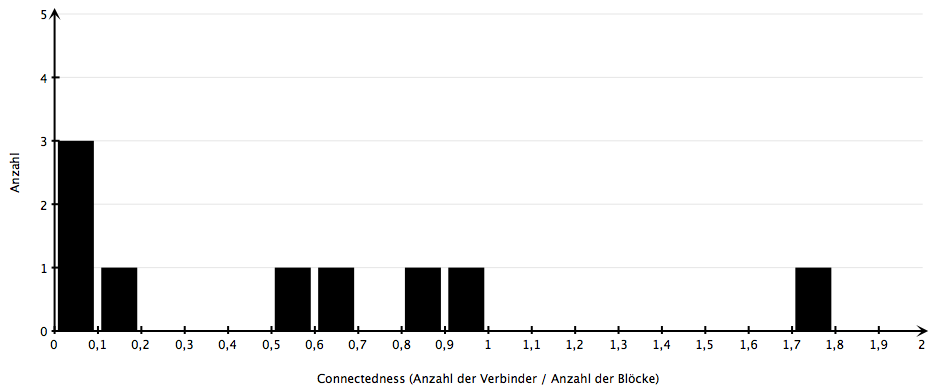
\includegraphics[height=2in]{img/Evaluierung/connectednessAushandlung1.png}
	\caption{Connectedness in Evaluierungsblock 2 - Durchgang 1}
	\label{fig:img_Evaluierung_connectednessAushandlung1}
\end{figure}

\begin{figure}[htbp]
	\centering
		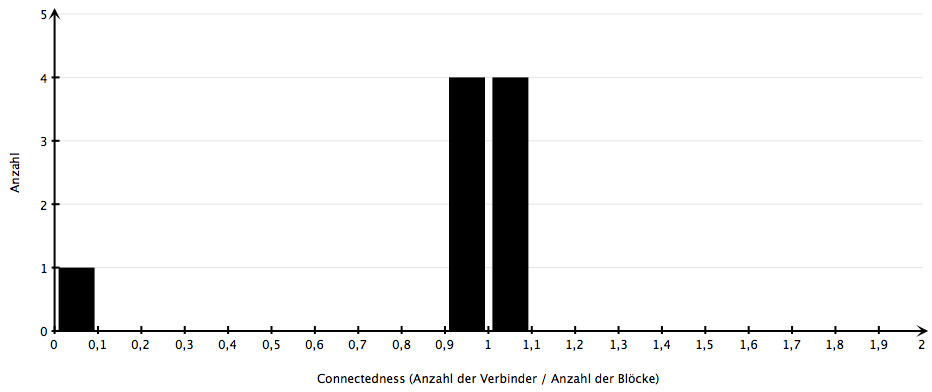
\includegraphics[height=2in]{img/Evaluierung/connectednessAushandlung2.png}
	\caption{Connectedness in Evaluierungsblock 2 - Durchgang 2}
	\label{fig:img_Evaluierung_connectednessAushandlung2}
\end{figure}

\begin{figure}[htbp]
	\centering
		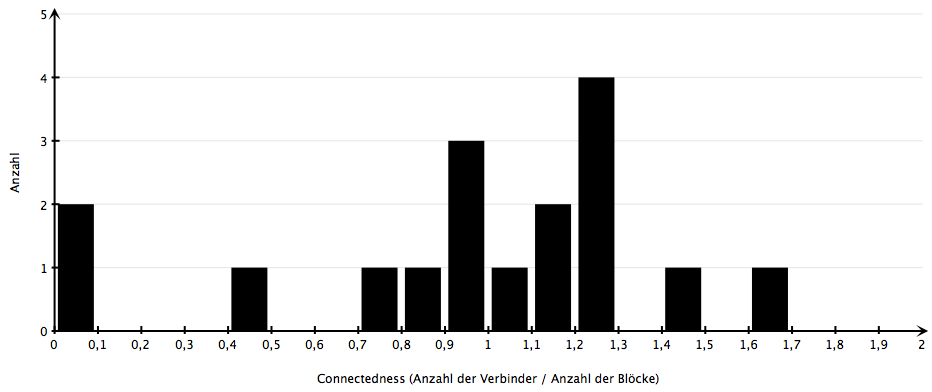
\includegraphics[height=2in]{img/Evaluierung/connectednessConceptMapping.png}
	\caption{Connctedness in Evaluierungsblock 3}
	\label{fig:img_Evaluierung_connectednessConceptMapping}
\end{figure}

Zu prüfen ist, ob die Connectedness in jenem Evaluierungs-Blöcken bzw. -Durchgängen, in denen die alternative Funktionalität zur Verbindungs-Herstellung verfügbar war, signifikant höher ist, als in jenen, in denen dies nicht der Fall war. Berechnet wird die Signifikanz zwischen den Ergebnissen der beiden Durchgänge von Block 2 ($conn_{B21}$ und $conn_{B22}$) sowie zwischen den Ergebnissen ersten Durchgang von Block 2 und den Ergebnissen von Block 3 ($conn_{B3}$). Im zweiten Fall ist zu beachten, dass die Aufgabenstellung nicht identisch war und somit eine potentielle Störvariable wirksam wird. Aufgrund der geringen Stichprobengröße kommt zur Prüfung der Signifikanz der t-Test nicht in Frage, es wird der \emph{Wilcoxon-Test} herangezogen. Der t-Test setzt außerdem Normalverteilung der Prüfgrößen voraus, was zumindest bei einer der Verteilungen nicht der Fall ist (Sharpiro-Wilk-Test für $conn_{B22}$: $p=6.29e^{-5}$, damit ist von Nicht-Normalverteilung auszugehen).

Die Null-Hypothese des Wilcoxon-Tests ist, das die beiden Verteilungen identisch verteilt sind. Entsprechend dem erwarteten Ergebnis (dass die mit der alternativen Funktionalität durchgeführten Anwendungen höhere Connectedness aufweisen) wurde die Alternativ-Hypothese so festgelegt, dass sie angenommen wird, wenn die Verteilung des zweiten Blocks gegenüber dem ersten Block nach rechts verschoben (also wertemäßig höher) ist.

Der Wilcoxon-Test für ungepaarte Stichproben ergibt für $conn_{B21}$ und $conn_{B22}$ und der eben beschriebenen Alternativ-Hypothese $p=0.9854$ -- die Alternativ-Hypothese ist damit anzunehmen, die zweite Verteilung (jene mit Einsatz der alternativen Funktionalität der Verbindungsherstellung) weist eine signifikant höhere Connectedness auf als die erste Verteilung (ohne diese Funktionalität). 

Für $conn_{B21}$ und $conn_{B3}$ ergibt der Wilcoxon-Test für ungepaarte Stichproben mit der gleichen Alternativ-Hypothese $p=0.98$ -- auch hier ist die Alternativ-Hypothese anzunehmen.

Für $conn_{B22}$ und $conn_{B3}$ ergibt der Wilcoxon-Test für ungepaarte Stichproben mit der gleichen Alternativ-Hypothese $p=0.7586$ -- auch hier ist die Alternativ-Hypothese anzunehmen.

\subsubsection{Diskussion} % (fold)

Aufgrund der Ergebnisse der berechneten Signifikanztests ist die Hypothese anzunehmen. Mit der Einführung der alternativen Möglichkeit zur Herstellung von Verbindungen war in den einzelnen Anwendungen des Werkzeugs eine Zunahme der Verwendung von Verbindern zu beobachten. Während die Benutzer bei der ursprünglichen Funktion zur Herstellung von Verbindungen zum Großteil auf diese verzichteten (auch bereits in Evaluierungsblock 1), wurden Verbinder unabhängig von der Aufgabenstellung mit der Einführung der alternativen Funktionalität verstärkt eingesetzt.

Die Connectedness eignet sich als Parameter zur vergleichenden Beurteilung des Ausmaßes der Verwendung von Verbindern, da durch die Einbeziehung der Größe des Modells (repräsentiert durch die Anzahl der verwendeten Modellelemente) in die Berechnung den Wert für unterschiedliche Modelle vergleichbar macht. 

Einfluss auf die Höhe der Connectedness hat aber die Aufgabenstellung, die zur Bildung des Modells führt. Unterschiedliche Modellierungsaufgaben führen zu unterschiedlichen Modell-Topologien, die sich wiederum in der Anzahl der verwendeten Verbinder auswirkt. Dies zeigt sich am Ergebnis des Wilcoxon-Tests für $conn_{B22}$ und $conn_{B3}$ -- in beiden Fällen stand die alternative Möglichkeit zur Verbindungsherstellung zur Verfügung $conn_{B3}$ ist trotzdem signifikant höher als $conn_{B22}$. Die kann darin begründet liegen, dass die Concept-Mapping-Aufgabe aus $conn_{B3}$ eher zu stärker verbundenen Modellen führt als eher zur ablauforientierten Modellen führende Arbeitsabstimmungs-Aufgabe aus $conn_{B22}$. Während bei Concept Mapping beliebige Konzepte in Beziehung stehen können, stehen Elemente bei ablauf-orientierten Modellen vor allem mit ihren kausalen Vorgängern und Nachfolgern in Beziehung, was die Anzahl der Verbinder einschränkt.

Aufgrund der großen Rolle der Aufgabenstellung ist bei der Überprüfung der Hypothese wichtig, diese Störvariable möglichst auszuschalten. Zur Beurteilung wird deswegen ausschließlich der Wilcoxon-Test zwischen $conn_{B21}$ und $conn_{B22}$ herangezogen, da in diese beiden Verteilungen mit der gleichen Aufgabenstellung und identischer Stichprobe (jedoch in zeitlichem Abstand von ca. einem Monat) zustande gekommen sind (da die Messungen unabhängig voneinander entstanden, wird ein Wilcoxon-Test für ungepaarte Variablen verwendet). Das Resultat des Wilcoxon-Tests spricht stark für die Annahme der Alternativhypothese des Tests und damit für die Annahme von Hypothese \ref{hyp:verbinder}. Zu berücksichtigen ist hier jedoch die geringe Stichprobengröße, die die Aussagekraft des Ergebnisses wieder in Frage stellt.

\subsubsection{Ergebnis} % (fold)

Die Auswertung zeigt eine signifikant höhere Verwendung von Verbindern bei Verfügbarkeit der alternativen Funktionalität zur Verbindungs-Herstellung. Auch die Natur der Aufgabenstellung scheint hohen Einfluss auf die Verwendung von Verbindern zu haben (siehe dazu auch die Diskussion von Hypothese \ref{hyp:keineverbinder} in Abschnitt XY). \textbf{Hypothese \ref{hyp:verbinder} kann auf Basis der vorliegenden Daten angenommen werden.}

% subsection herstellung_von_verbindern (end)

\subsection{Verwendung des Löschtokens} % (fold)
\label{sub:verwendung_des_löschtokens}

In diesem Abschnitt werden die Ergebnisse der Überprüfung der Hypothese \ref{hyp:radierer} („Das Löschtoken ermöglicht intuitives Löschen von Modellelementen.“) vorgestellt.

\subsubsection{Auswertung} % (fold)

\begin{transkript}
	\emph{Die Teilnehmer möchten einen Block umbenennen.}\\
	\textbf{A:} Wie haben wir jetzt gesagt \emph{(markiert den roten Baustein)} keine Modellierungsvorgabe \emph{(gibt Bezeichnung ein)}\\
	\emph{System übernimmt die neue Beschriftung für den Baustein nicht.}\\
	\textbf{A:} Wo wurde das hingeschrieben? \emph{(Pause)} Radiergummi? Glaubst du kann man das wegradieren?\\
	\textbf{B:} Probiere es aus.\\
	\textbf{\emph{A legt Radiergummi zum Block mit der Absicht die Beschriftung zu löschen}}\\
	\textbf{B:} Nein! Du löscht alles. Hör auf! \\
	\textbf{A:} Ok wie war das zuerst? Lassen wir das mal weg. \emph{(legt Baustein zur Seite)}\\
	\emph{A legt den Block zur Seite.} 
\end{transkript}

Ein ähnliches Missverständnis zeigt sich auch in folgender Situation:

\begin{transkript}
	\emph{TLN A und B stellen jeweils ihren Marker zu den Blöcken, die verbunden werden sollen. Dabei wird eine gerichtete Verbindung erstellt.}\\
	\textbf{C:} Jetzt haben wir aber einen Pfeil gebastelt.\\
	\textbf{B:} Ja stimmt. Interessant.\\
	\textbf{A:} Wie war das mit dem Radiergummi. \emph{(nimmt Radiergummi und legt ihn auf die Verbindung)}\\
	\textbf{B:} Nein\\
	\textbf{C:} Nein, mit dem Glas! Du löscht alles!\\
	\textbf{A:} Nein nur die Verbindung. \textbf{\emph{(Macht Radierbewegungen auf der Verbindung)}}\\
	\textbf{C:} Ich glaube dass wir das Glas nehmen müssen.\\
	\emph{A schiebt die Blöcke zwischen denen die Verbindung gelöscht werden soll zusammen.}\\
	\textbf{A:} Da es funktioniert. \emph{(schiebt die Blöcke weiter auseinander und bemerkt dass die Verbindung nicht gelöscht wurde)} Nein.\\
	\textbf{B:} Ich glaube der Radiergummi vernichtet alles.\\
	\textbf{A:} Nein der Radiergummi vernichtet nur Verbindungen. Nur welche? \emph{(schiebt beide Blöcke wieder zusammen – nimmt Radiergummi weg und schiebt Blöcke in die Ausgangsposition)}
\end{transkript}

\begin{transkript}
	\emph{Es wird eine falsche Beschriftung eingefügt. Die Teilnehmer wollen diese löschen, verwenden den Radiergummi allerdings falsch.}\\
	\textbf{B:} Aber irgendwie steht jetzt Ereignisse nicht bei dem Ding \emph{(zeigt auf gelben Block)} sondern dort \emph{(zeigt auf beschriftete Verbindung)}.\\
	\emph{A verrückt den gelben Block ein wenig.}\\
	\textbf{B:} Normal ist das nicht oder?\\
	\textbf{C:} Nein.\\
	\emph{A nimmt den Radiergummi.}\\
	\textbf{A:} Ich glaube das. \emph{(setzt den Radiergummi auf die Arbeitsfläche)}\\
	\textbf{C:} Aber nicht alles!\\
	\emph{A nimmt Radiergummi wieder weg. System erstellt eine Verbindung zwischen zwei roten Blöcken. Teilnehmer lachen. \textbf{A legt Radiergummi auf die erstellte Verbindung, und nimmt ihn wieder weg.} A nimmt die beiden verbundenen Blöcke und verschiebt sie.}\\
	\textbf{A:} Vielleicht so. \emph{(führt die Blöcke zusammen)}
\end{transkript}

\begin{transkript}
	\emph{In der Szene erstellt das System einen ungewollten Verbinder, die Teilnehmer versuchen auf verschiedene Arten den Verbinder zu löschen.}\\
	\textbf{B:} Und wie kann ich die Verbindungen löschen?\\
	\textbf{B:} Warte einmal, da gibt es irgendwo das mit dem Radiergummi.\\
	\textbf{A:} murmelt zustimmend \\
	\emph{\textbf{B nimmt den Radiergummi und platziert ihn direkt auf dem Verbinder}}\\
	\emph{Das System färbt den Tisch rot}\\
	\textbf{A:} Nein, warte. Da löscht du Alles!\\
	\emph{\textbf{B verschiebt den Radiergummi auf dem Tisch, hebt ihn an und platziert ihn direkt auf einem Block.}}\\
	\emph{Sobald der Radiergummi von der Oberfläche auf den Block gelegt wurde, entfernt das System die rote Färbung.}\\
	\textbf{A:} Ich glaube da löscht du Alles.\\
	\emph{B legt den Radiergummi an mehreren Stellen trotz der Warnung von TN A auf die Oberfläche}\\
	\textbf{B:} Nein, es will eh nicht.\\
\end{transkript}

\begin{transkript}
	\emph{C versucht die Benennung eines Verbinders mittels Radiergummi zu entfernen.}\\
	\textbf{B:} Aber irgendwie steht jetzt Ereignisse nicht bei dem Ding \emph{(deutet auf einen Block)} sondern dort \emph{(deutet auf einen Verbinder)}. Das wollen wir nicht oder?\\
	\textbf{A:} Nein.\\
	\textbf{C:} Ich glaube das. \emph{\textbf{(nimmt den Radiergummi und legt ihn auf den Verbinder den die Teilnehmer entfernen wollen.)}}\\
	\textbf{A:} Aber nicht alles.\\
	\emph{C entfernt den Radiergummi wieder von der Modellierungsoberfläche. In diesem Moment erstellt das System automatisch einen neuen Verbinder. C versucht den neuen Verbinder mittels Radiergummi zu entfernen.}\\
	\textbf{A:} Oh Gott.\\
	\textbf{C:} Vielleicht so \emph{(schiebt die beiden betroffenen Blöcke zusammen)}, nein.\\
	\textbf{B:} Nein.\\
	\textbf{A:} Oh Gott oh Gott oh Gott.\\
	\textbf{B:} Gehen wir einen Prozessschritt zurück.\\
	\textbf{C:} Genau.\\
\end{transkript}

\begin{transkript}
	\emph{Teilnehmer versuchen mit dem Radiergummi und nur einem anderen Marker einen Verbinder zu entfernen.}\\
	\textbf{B:} Können wir die nicht so auch einfach löschen?\\
	\textbf{C:} Ja mit dem Radiergummi.\\
	\textbf{B:} Muss ich den jetzt zuerst so \emph{(Hält den Radiergummi zur Kamera)} hinhalten?\\
	\textbf{A:} Nein, ich glaube, \textbf{den musst du einfach da \emph{(zeigt auf den Verbinder)} drauf legen.}\\
	\emph{B legt den Radiergummi auf den vom System automatisch erstellten Verbinder.}\\
	\textbf{A:} Und jetzt muss man \emph{(legt ein Markierungtoken auf den Verbinder)} Nein.\\
	\emph{Der Verbinder lässt sich auf diese Art nicht löschen und die Teilnehmer entscheiden sich den Fehler mittels der Wiederherstellungsfunktion zu beseitigen.}
\end{transkript}

\subsubsection{Diskussion} % (fold)

\subsubsection{Ergebnis} % (fold)

% subsection verwendung_des_löschtokens (end)
% section ergebnisse (end)

% chapter eval_tui (end) 